\PassOptionsToPackage{unicode=true}{hyperref} % options for packages loaded elsewhere
\PassOptionsToPackage{hyphens}{url}
\PassOptionsToPackage{dvipsnames,svgnames*,x11names*}{xcolor}
%
\documentclass[10pt,ignorenonframetext,]{beamer}
\usepackage{pgfpages}
\setbeamertemplate{caption}[numbered]
\setbeamertemplate{caption label separator}{: }
\setbeamercolor{caption name}{fg=normal text.fg}
\beamertemplatenavigationsymbolsempty
% Prevent slide breaks in the middle of a paragraph:
\widowpenalties 1 10000
\raggedbottom
\setbeamertemplate{part page}{
\centering
\begin{beamercolorbox}[sep=16pt,center]{part title}
  \usebeamerfont{part title}\insertpart\par
\end{beamercolorbox}
}
\setbeamertemplate{section page}{
\centering
\begin{beamercolorbox}[sep=12pt,center]{part title}
  \usebeamerfont{section title}\insertsection\par
\end{beamercolorbox}
}
\setbeamertemplate{subsection page}{
\centering
\begin{beamercolorbox}[sep=8pt,center]{part title}
  \usebeamerfont{subsection title}\insertsubsection\par
\end{beamercolorbox}
}
\AtBeginPart{
  \frame{\partpage}
}
\AtBeginSection{
  \ifbibliography
  \else
    \frame{\sectionpage}
  \fi
}
\AtBeginSubsection{
  \frame{\subsectionpage}
}
\usepackage{lmodern}
\usepackage{amssymb,amsmath}
\usepackage{ifxetex,ifluatex}
\usepackage{fixltx2e} % provides \textsubscript
\ifnum 0\ifxetex 1\fi\ifluatex 1\fi=0 % if pdftex
  \usepackage[T1]{fontenc}
  \usepackage[utf8]{inputenc}
  \usepackage{textcomp} % provides euro and other symbols
\else % if luatex or xelatex
  \usepackage{unicode-math}
  \defaultfontfeatures{Ligatures=TeX,Scale=MatchLowercase}
\fi
\usetheme[]{Singapore}
\usefonttheme{serif}
% use upquote if available, for straight quotes in verbatim environments
\IfFileExists{upquote.sty}{\usepackage{upquote}}{}
% use microtype if available
\IfFileExists{microtype.sty}{%
\usepackage[]{microtype}
\UseMicrotypeSet[protrusion]{basicmath} % disable protrusion for tt fonts
}{}
\IfFileExists{parskip.sty}{%
\usepackage{parskip}
}{% else
\setlength{\parindent}{0pt}
\setlength{\parskip}{6pt plus 2pt minus 1pt}
}
\usepackage{xcolor}
\usepackage{hyperref}
\hypersetup{
            pdftitle={Klyngeanalyse},
            pdfauthor={Stefanie Muff, Institutt for matematiske fag},
            colorlinks=true,
            linkcolor=Maroon,
            filecolor=Maroon,
            citecolor=Blue,
            urlcolor=blue,
            breaklinks=true}
\urlstyle{same}  % don't use monospace font for urls
\newif\ifbibliography
\usepackage{longtable,booktabs}
\usepackage{caption}
% These lines are needed to make table captions work with longtable:
\makeatletter
\def\fnum@table{\tablename~\thetable}
\makeatother
\usepackage{graphicx,grffile}
\makeatletter
\def\maxwidth{\ifdim\Gin@nat@width>\linewidth\linewidth\else\Gin@nat@width\fi}
\def\maxheight{\ifdim\Gin@nat@height>\textheight\textheight\else\Gin@nat@height\fi}
\makeatother
% Scale images if necessary, so that they will not overflow the page
% margins by default, and it is still possible to overwrite the defaults
% using explicit options in \includegraphics[width, height, ...]{}
\setkeys{Gin}{width=\maxwidth,height=\maxheight,keepaspectratio}
\setlength{\emergencystretch}{3em}  % prevent overfull lines
\providecommand{\tightlist}{%
  \setlength{\itemsep}{0pt}\setlength{\parskip}{0pt}}
\setcounter{secnumdepth}{0}

% set default figure placement to htbp
\makeatletter
\def\fps@figure{htbp}
\makeatother

\usepackage{multicol}

\title{Klyngeanalyse}
\providecommand{\subtitle}[1]{}
\subtitle{ISTx1003 Statistisk læring og Data Science}
\author{Stefanie Muff, Institutt for matematiske fag}
\date{November 12, 2021}

\begin{document}
\frame{\titlepage}

\begin{frame}{Plan for i dag}
\protect\hypertarget{plan-for-i-dag}{}

\(~\)

\begin{itemize}
\item
  Hva er klyngeanalyse
\item
  Læringsmål, pensum og læringsressurser
\item
  Avstandsmål
\item
  K-gjennomsnitt (``K-means'') klyngeanalyse
\item
  Bruk av klyngeanalyse på et bilde (prosjektet fra i fjor)
\item
  Hierarkisk klyngeanalyse
\item
  Informasjon om prosjektet
\end{itemize}

\end{frame}

\begin{frame}{Eksempel 1: Genaktivitet}
\protect\hypertarget{eksempel-1-genaktivitet}{}

\begin{itemize}
\item
  \(n=81\) celleprøver fra kreftsvulster til ulike pasienter
\item
  genaktivitet for \(p =12957\) gener
\end{itemize}

\vspace{2mm}

\textbf{Spørsmål:}

Hvilke celleprøver fra brystkreftpasienter ligner hverandre mest?

Kan vi finne ukjente klynger (av celleprøver) i dataene?

Dette kan hjelpe for å forutse sannsynligheten for en tilbakefall.

\end{frame}

\begin{frame}

\centering

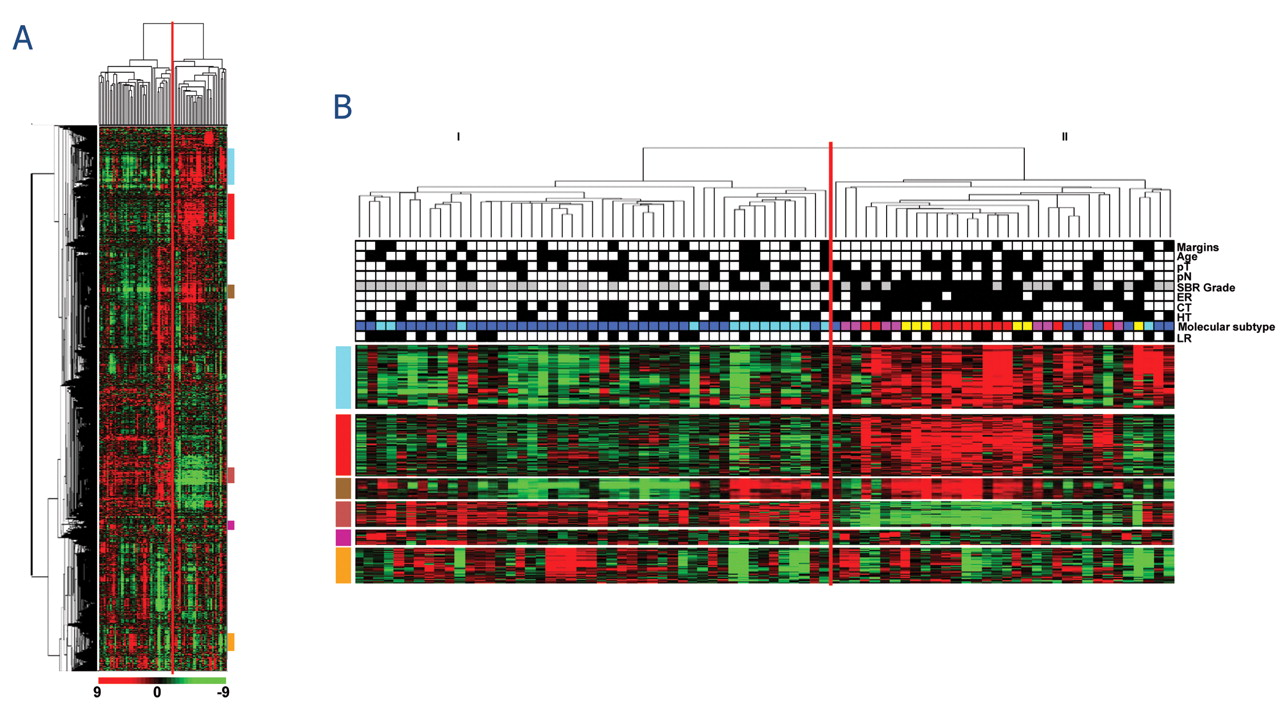
\includegraphics[width=0.9\textwidth,height=\textheight]{gene_expression.jpg}
\[ X = p\times n  =  \text{gener} \times \text{prøver}  \ .\]

\tiny

Finn ut mer: \url{https://cgp.iiarjournals.org/content/8/4/199}

\end{frame}

\begin{frame}{Eksempel 2: Proteininteraksjonsnettwerk}
\protect\hypertarget{eksempel-2-proteininteraksjonsnettwerk}{}

Kan vi finne klynger med relatert funksjon?

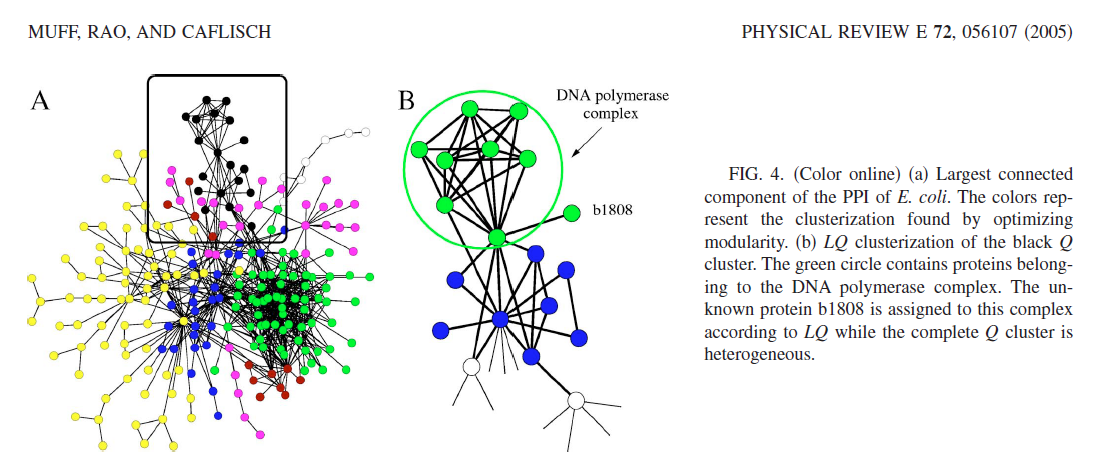
\includegraphics{muff_etal.png}

\end{frame}

\begin{frame}{Eksempel 3: Bildanalyse}
\protect\hypertarget{eksempel-3-bildanalyse}{}

Det var en prosjektoppgave i fjor.

Mål:

Å bruke klyngeanalyse til å fjerne detaljer og støy - ved å dele
pikslene inn i to eller flere klynger.

Todo: Ev adapt with task from this year.

\end{frame}

\begin{frame}{Læringsmål}
\protect\hypertarget{luxe6ringsmuxe5l}{}

\begin{itemize}
\item
  forstå hvorfor det er interessant å gjøre klyngeanalyse
\item
  kjenne igjen situasjoner der klyngeanalyse vil være en aktuell metode
  å bruke
\item
  kjenne begrepene avstandsmål, koblingstype, dendrogram
\item
  forstå algoritmen for å utføre K-gjennomsnitt-klyngeanalyse og
  hierarkisk klyngeanalyse
\item
  forstå hvordan klyngeanalyse utføres i Python
\item
  kunne besvare oppgave 3 av prosjektoppgaven på en god måte!
\end{itemize}

\end{frame}

\begin{frame}{Læringsressurser}
\protect\hypertarget{luxe6ringsressurser}{}

\vspace{2mm}

\(~\)

Tema Klyngeanalyse:

\vspace{2mm}

\begin{itemize}
\item
  \textbf{Kompendium}: Klyngeanalyse (pdf og html, by Mette Langaas)
\item
  \textbf{Korte videoer}: (by Mette Langaas)

  \begin{itemize}
  \tightlist
  \item
    Klyngeanalyse (8:43 min)
  \item
    Hierarkisk klyngeanalyse (11:26 min)
  \item
    K-gjennomsnitt-klyngeanalyse (8:38 min)
  \end{itemize}
\item
  Denne forelesningen
\item
  \textbf{Disse slides} med notater
\end{itemize}

\(~\)

Som alltid se her:

\url{https://wiki.math.ntnu.no/istx1003/2021h/start}

\end{frame}

\begin{frame}{Klyngeanalyse -- hva er det?}
\protect\hypertarget{klyngeanalyse-hva-er-det}{}

Vi har data \[X : n\times p\] men \emph{ikke} noen respons \(Y\).
\emph{\textcolor{red}{Ikke-veiledet = unsupervised}}

\vspace{4mm}

\textbf{Mål:}

\begin{itemize}
\tightlist
\item
  Finn ukjente klynger i dataene.
\item
  Observasjoner innen hver klynge er mer lik hverandre enn observasjoner
  fra ulike klynger.
\end{itemize}

\vspace{2mm}

\textbf{Hva skal vi bruke resultatene fra klyngeanalysen til?}

\begin{itemize}
\tightlist
\item
  Bildet: Fjerne støy eller, spare lagringsplass
\item
  Medisin: Finne subgrupper av en sykdom \(\rightarrow\) relevant for
  behandling?
\end{itemize}

\vspace{2mm}

\end{frame}

\begin{frame}{Klyngeanalyse -- hva er det?}
\protect\hypertarget{klyngeanalyse-hva-er-det-1}{}

\textbf{Generelt}: Finne \emph{\textcolor{red}{struktur}} i dataene.

\vspace{6mm}

Kan vi stole på resultatene? Hvor robuste er de?

\(\rightarrow\) Fortsatt et forskningsområde!

\end{frame}

\begin{frame}{Avstandsmål}
\protect\hypertarget{avstandsmuxe5l}{}

Før en klyngeanalyse må vi først definere en \emph{avstand} mellom to
datapoeng.

To populære avstandsmal:

\textbf{Euklidsk} \hspace{4cm} \textbf{City-block (=Manhattan)}

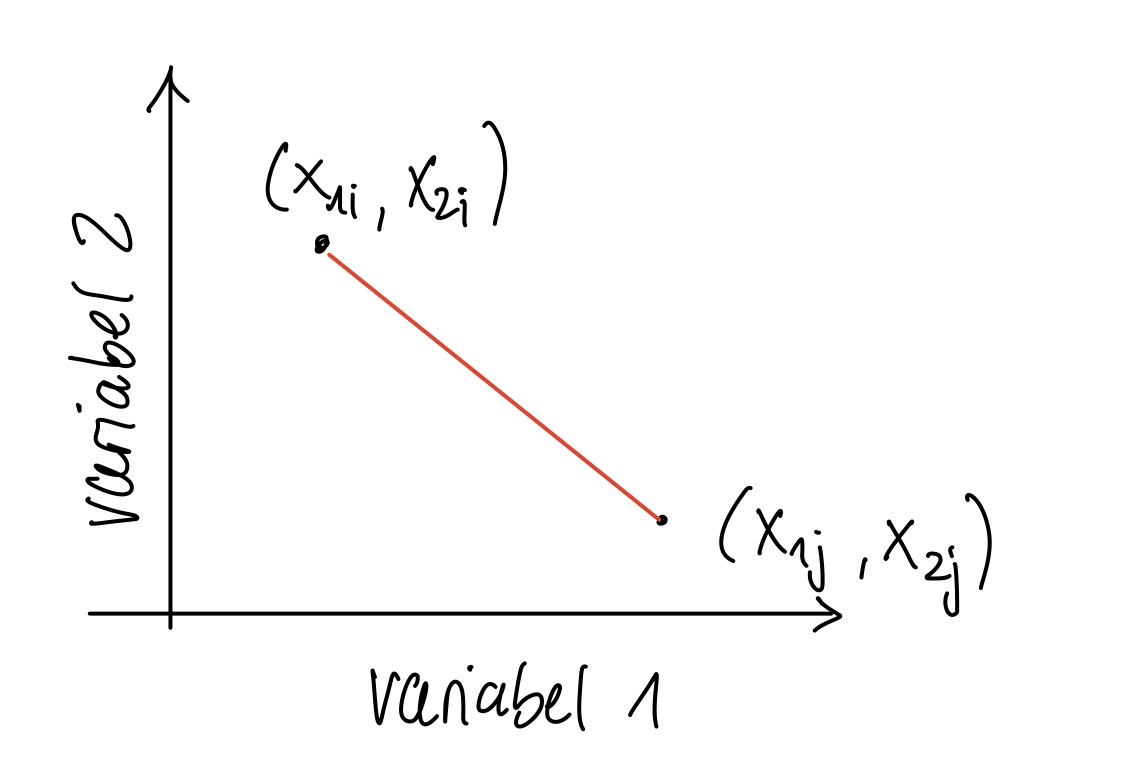
\includegraphics[width=0.48\textwidth,height=\textheight]{euklid.png}
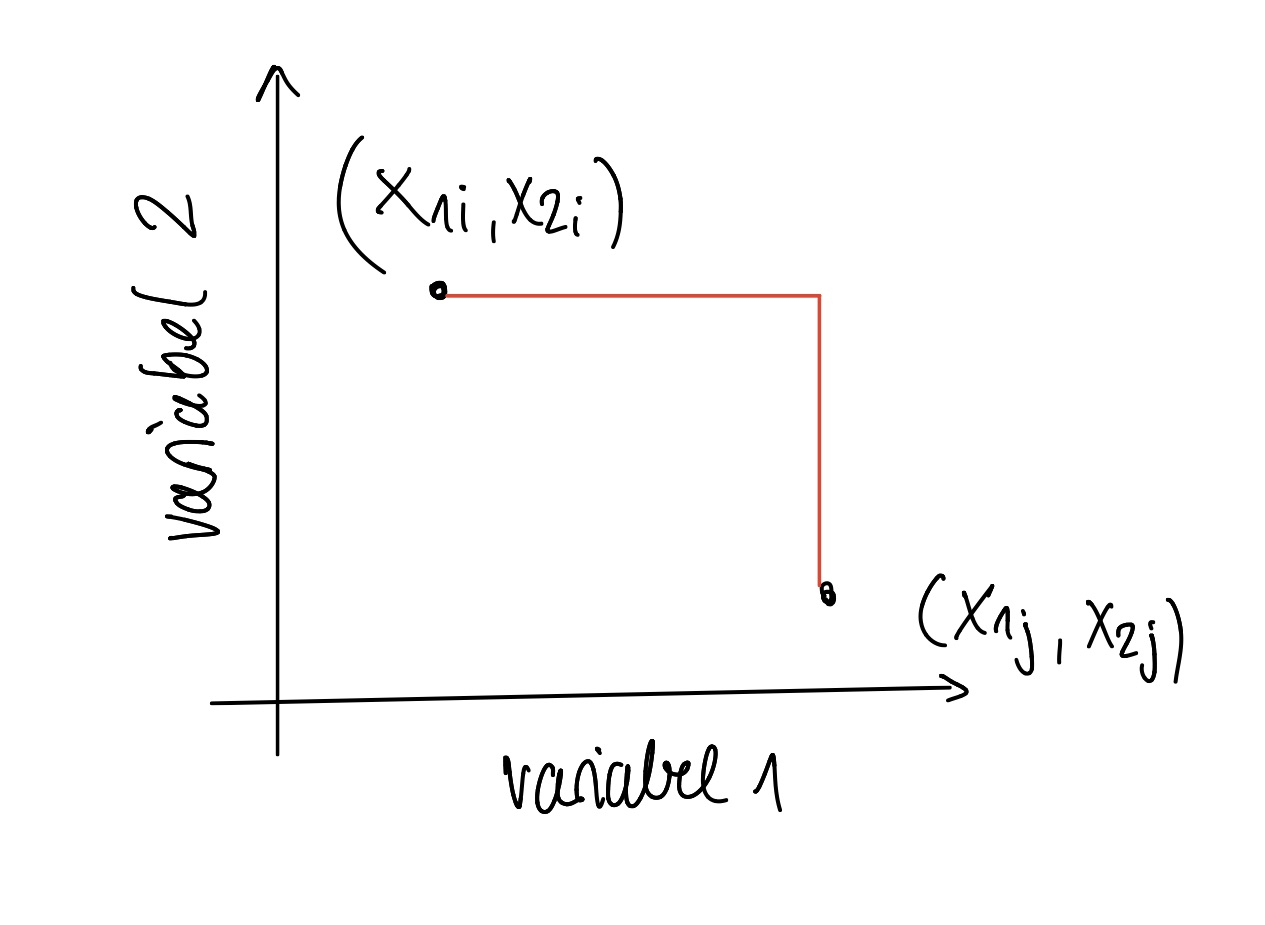
\includegraphics[width=0.5\textwidth,height=\textheight]{manhattan.png}

\end{frame}

\begin{frame}

\textbf{Euklidsk} \hspace{4cm} \textbf{City-block (=Manhattan)}

\[D_E(i,i') = \sqrt{\sum_{j=1}^p (x_{ji} - x_{ji'})^2} \qquad \quad D_M(i,i') =  \sum_{j=1}^p |x_{ji} - x_{ji'}|\]

\(~\)

Avstandsmål i mer enn 2 dimensioner: Enkelt å regne, men litt vanskelig
å forestille seg.

\end{frame}

\begin{frame}{Metoder for klyngeanalyse}
\protect\hypertarget{metoder-for-klyngeanalyse}{}

Det fins ganske mange metoder, men vi ser på to som er (mest?) populær:

\textbf{K-gjennomsnitt klyngeanalyse}

\centering

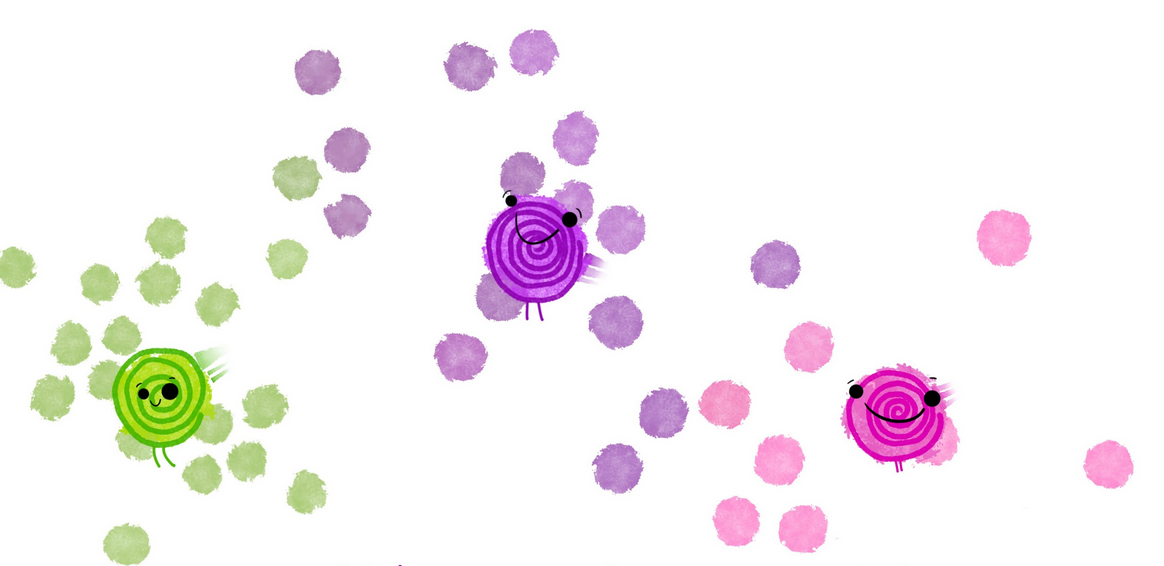
\includegraphics[width=0.5\textwidth,height=\textheight]{kmeans_AllisonHorst.png}

\flushleft

\textbf{Hierarkisk klyngeanalyse}

\centering

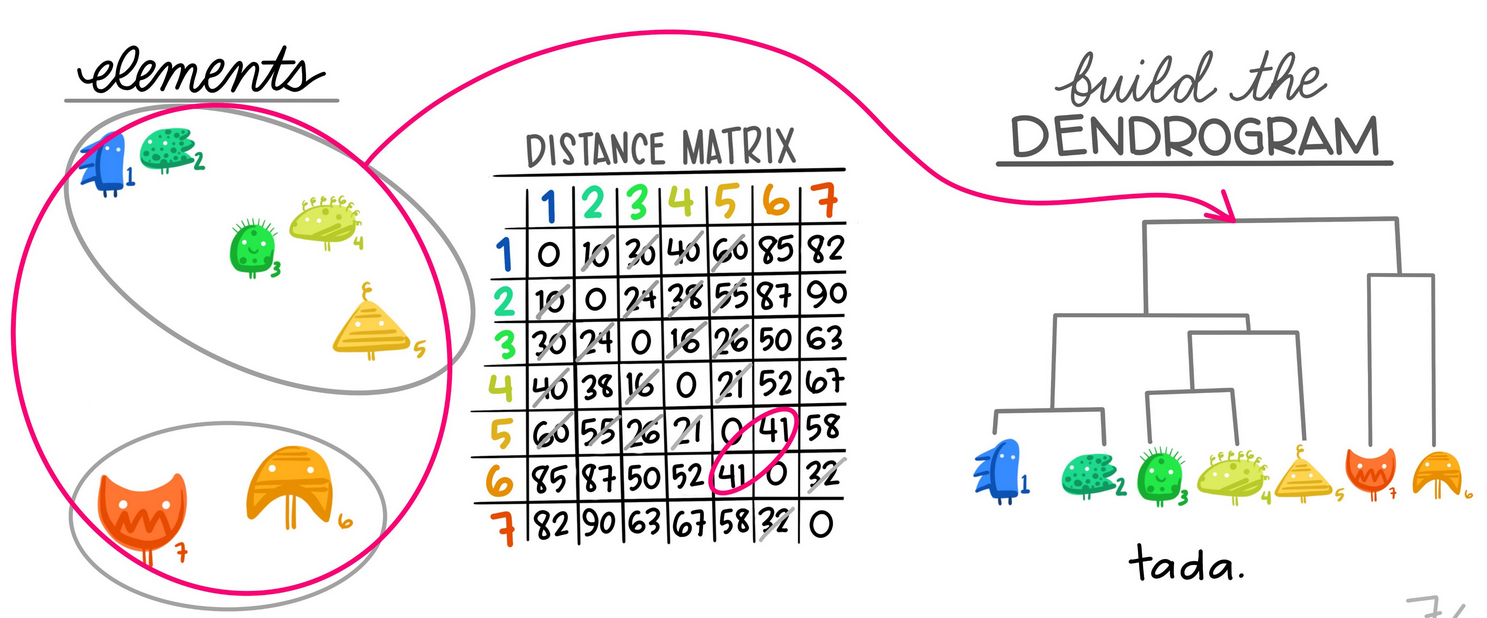
\includegraphics[width=0.55\textwidth,height=\textheight]{hierclust_AllisonHorst.png}

\tiny Artwork by @allison\_horst

\end{frame}

\begin{frame}

\begin{block}{K-gjennomsnitt klyngeanalyse}

\(~\)

\begin{itemize}
\tightlist
\item
  Finn \(K\) ukjente klynger i dataene.
\end{itemize}

\vspace{2mm}

\centering

\includegraphics[width=0.5\linewidth]{3Klyngeanalyse_files/figure-beamer/unnamed-chunk-1-1}

\begin{itemize}
\tightlist
\item
  Alle observasjoner skal være medlem i akkurat en klynge
\item
  Variasjonen innen hver klynge skal være så liten som mulig
\end{itemize}

\end{block}

\end{frame}

\begin{frame}

\begin{block}{Variasjon innen en klynge \(k\)}

\(~\)

\begin{itemize}
\item
  \(K\) klynger \(C_1, \ldots, C_k, \ldots, C_K\).
\item
  Antall observasjoner i klynge \(k\): \(|C_k|\).
\item
  Variasjon in klynge \(k\):
  \[\frac{1}{|C_k|} \sum_{i,i'\in C_k}\sum_{j=1}^p (x_{ij}-x_{i'j})^2\]
\end{itemize}

\(~\)

\textbf{Optimeringsproblem}

Vi vil \emph{minimere} variasjon over \emph{alle klynger}:
\[\sum_{k=1}^K\frac{1}{|C_k|} \sum_{i,i'\in C_k}\sum_{j=1}^p (x_{ij}-x_{i'j})^2\]

\end{block}

\end{frame}

\begin{frame}

Nyttig sammenhang som er grunnlag for \(k\)-gjennomsnitt algoritme

\[\sum_{k=1}^K\frac{1}{|C_k|} \sum_{i,i'\in C_k}\sum_{j=1}^p (x_{ij}-x_{i'j})^2\]

\[ = \sum_{k=1}^K 2 \sum_{i\in C_k}\sum_{j=1}^p (x_{ij}-\overline{x}_{kj})^2\ ,\]
\(~\)

med \emph{klyngesentroide} i klynge \(k\):
\(\overline{x}_k = (\overline{x}_{k1}, \ldots, \overline{x}_{kp})\)

\end{frame}

\begin{frame}

\begin{block}{K-gjennomsnitt algoritme}

\(~\)

\begin{itemize}
\tightlist
\item
  Start med å velge antall klynker \(K\).
\end{itemize}

\vspace{2mm}

\begin{itemize}
\item
  Tilordne hver observasjon til en klynge

  \begin{itemize}
  \tightlist
  \item
    Mange muligheter

    \begin{itemize}
    \tightlist
    \item
      tilfeldig velge ut \(K\) observasjoner og sette disse som
      klyngesentroider
    \item
      tilfeldig klynger
    \end{itemize}
  \item
    og deretter tilordne der resterende observasjoner til klyngen med
    nærmeste klyngesentroide.
  \end{itemize}
\end{itemize}

\vspace{2mm}

\begin{itemize}
\tightlist
\item
  \textcolor{red}{Repeter} (iterativt) \emph{til ingen observasjoner
  endrer klyngemedlemskap}:

  \begin{enumerate}
  \tightlist
  \item
    For hver klynge regn ut klyngesentroiden
  \item
    Tilordne hver observasjon til klyngen til nærmeste klyngesentroide
  \end{enumerate}
\end{itemize}

\end{block}

\end{frame}

\begin{frame}

\begin{block}{Illustrasjon av \(K\)-gjennomsnitt algoritme (\(K=3\))}

\centering

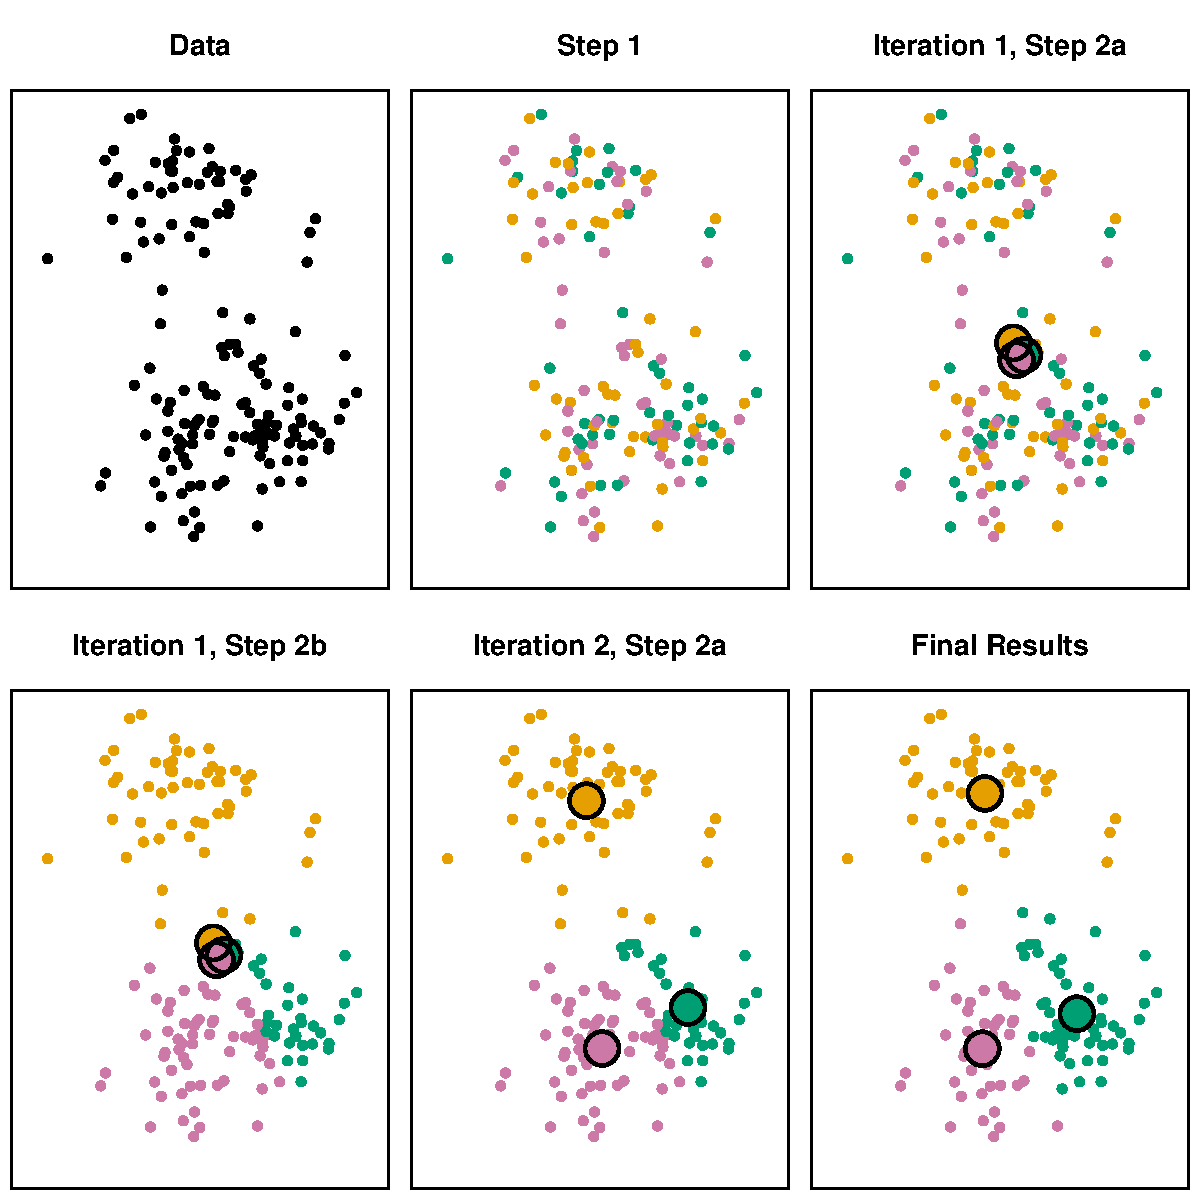
\includegraphics[width=0.7\textwidth,height=\textheight]{10.6.pdf}

\scriptsize

Fig. 10.6 fra ``An Introduction to Statistical Learning with
Applications in R'', James et al 2013.

\end{block}

\end{frame}

\begin{frame}

\begin{block}{\(K\)-gjennomsnitt-algoritmen i Python}

Todo

\end{block}

\end{frame}

\begin{frame}

\begin{block}{Prosjektoppgaven}

Todo

\end{block}

\end{frame}

\begin{frame}{Hierarkisk klyngeanalyse}
\protect\hypertarget{hierarkisk-klyngeanalyse}{}

\(~\)

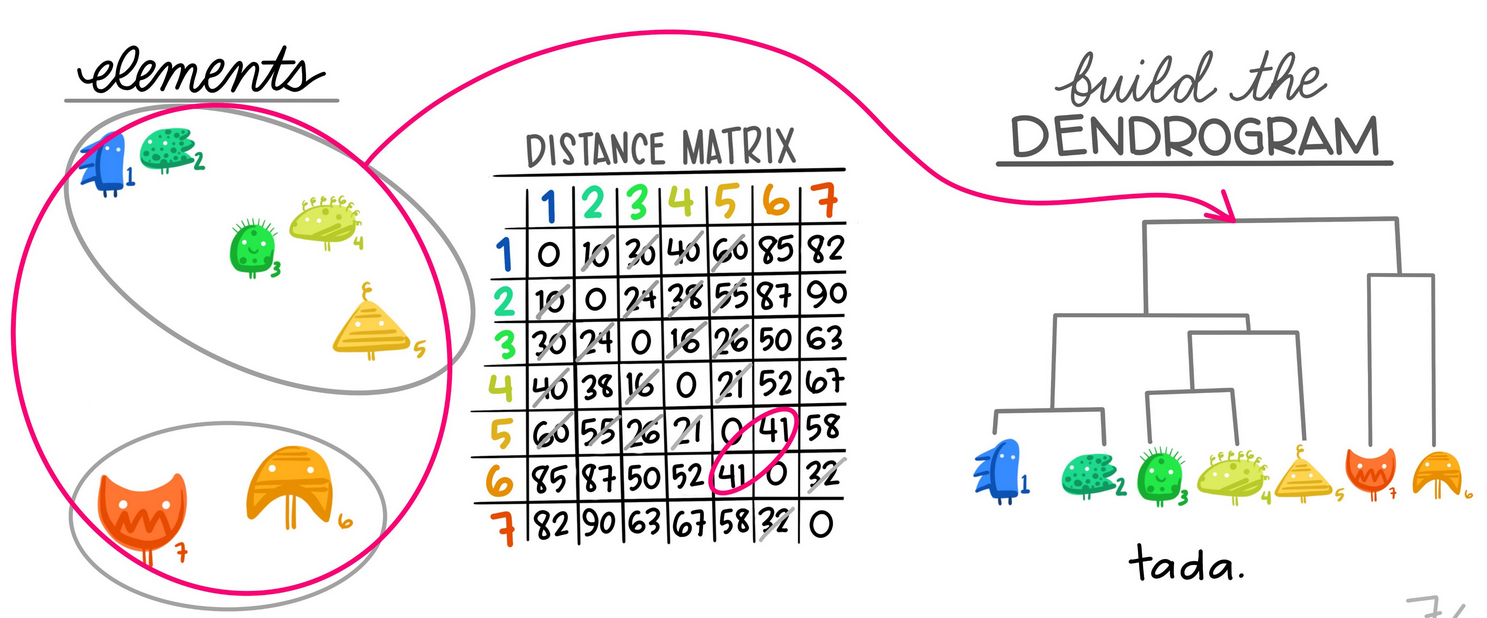
\includegraphics[width=0.8\textwidth,height=\textheight]{hierclust_AllisonHorst.png}

\tiny Artwork by @allison\_horst

\end{frame}

\begin{frame}

\begin{block}{Eksempel}

\(~\)

\(n=5, p=2\)

\(~\)

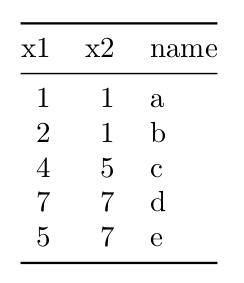
\includegraphics[width=0.25\textwidth,height=\textheight]{table.png}
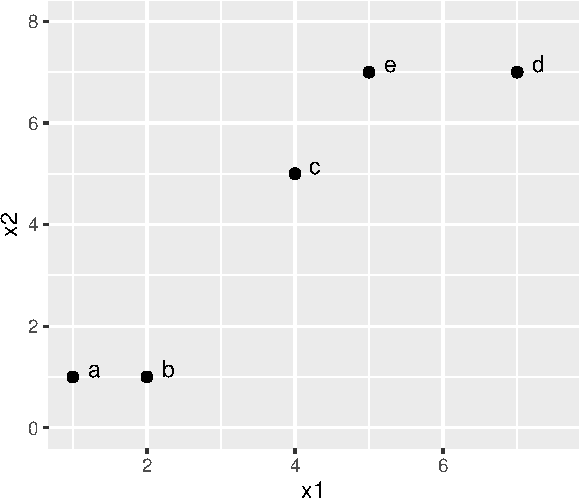
\includegraphics[width=0.65\textwidth,height=\textheight]{exampleplot-1.pdf}

\end{block}

\end{frame}

\begin{frame}

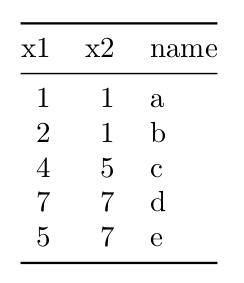
\includegraphics[width=0.25\textwidth,height=\textheight]{table.png}
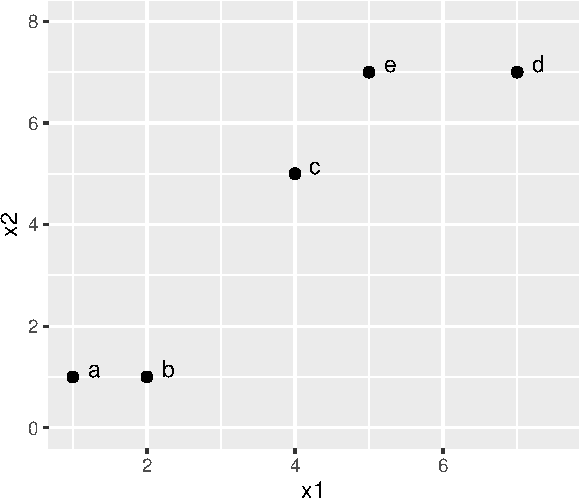
\includegraphics[width=0.65\textwidth,height=\textheight]{exampleplot-1.pdf}

\begin{enumerate}
[1)]
\tightlist
\item
  Velg avstandsmål
\item
  Regn ut avstanden mellom alle par av observasjoner
\item
  Plasser avstandene inn i en \(n\times n\) matrise
\end{enumerate}

\end{frame}

\begin{frame}

\begin{block}{Avstandsmatrise (Euklidsk avstand)}

\(~\)

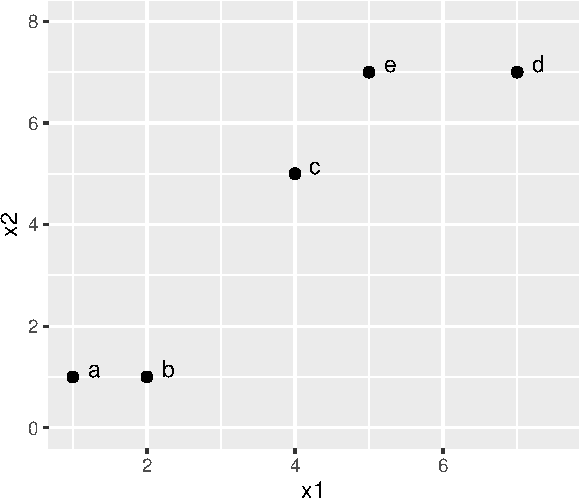
\includegraphics[width=0.5\textwidth,height=\textheight]{exampleplot-1.pdf}

\begin{longtable}[]{@{}cccccc@{}}
\toprule
name & a & b & c & d & e\tabularnewline
\midrule
\endhead
a & 0.0 & 1.0 & 5.0 & 8.5 & 7.2\tabularnewline
b & 1.0 & 0.0 & 4.5 & 7.8 & 6.7\tabularnewline
c & 5.0 & 4.5 & 0.0 & 3.6 & 2.2\tabularnewline
d & 8.5 & 7.8 & 3.6 & 0.0 & 2.0\tabularnewline
e & 7.2 & 6.7 & 2.2 & 2.0 & 0.0\tabularnewline
\bottomrule
\end{longtable}

\end{block}

\end{frame}

\end{document}
